%General Class Template
\documentclass[12pt]{article}
%Packages to load which give you useful commands
\usepackage{amsmath,amsthm}			% want AMS fonts
\usepackage{amssymb}
\usepackage{lastpage}
\usepackage[pdftex]{graphicx}			% for including images
\usepackage{hyperref}				% for links
\usepackage{epstopdf}
\usepackage{setspace}
\usepackage{tikz}
\usepackage{enumerate}
%\doublespacing
\usepackage{fullpage}
% \usepackage{tkz-graph}
% \usetikzlibrary{shapes.geometric}

\tikzstyle{vertex}=[circle, draw, fill=black, inner sep=0pt, minimum size=1pt]
\newcommand{\vertex}{\node[vertex]}

\renewcommand{\O}{\mathcal{O}}
\newcommand{\D}{\mathcal{D}}
\renewcommand{\H}{\mathcal{H}}
\newcommand{\C}{\mathcal{C}}
\newcommand{\I}{\mathcal{I}}
\newcommand{\w}{\textrm{width}}

\newcommand{\N}{\mathbb{N}}
\newcommand{\Z}{\mathbb{Z}}
\newcommand{\Q}{\mathbb{Q}}
\newcommand{\R}{\mathbb{R}}
\newcommand{\makeset}[2]{ \{#1\;|\;#2\} }

\def\mchoose#1#2{\left(\kern-.2em\binom{#1}{#2}\kern-.2em\right)}
%Sets the margins: I like lots of space for text
\textwidth = 7 in
\textheight = 9.5 in
\oddsidemargin = -0.3 in
\evensidemargin = -0.3 in
\topmargin = -0.4 in
\headheight = 0.0 in
\headsep = 0.0 in
\parskip = 0.2in
\parindent = 0.0in

%defines a few theorem-type environments
\newcommand{\hooray}[1]{#1}
\newtheorem{theorem}{Theorem}
\newtheorem{lemma}[theorem]{Lemma}
\newtheorem{corollary}[theorem]{Corollary}
\newtheorem{proposition}[theorem]{Proposition}
\newtheorem{problem}[theorem]{Problem}
\newtheorem{case}[theorem]{Case}
\newtheorem{subcase}[theorem]{SubCase}
\newtheorem{transrule}[theorem]{TransRule}
\newtheorem{branchrule}[theorem]{BranchRule}
\newtheorem{remark}[theorem]{Remark}
\newtheorem{fact}[theorem]{Fact}
\newtheorem{definition}[theorem]{Definition}

\begin{document}
	{ \hfill Math Camp Day 1 Lecture 1 Lesson Plan
\hfill
\today}
\section*{Learning Objectives/Goals}
\begin{itemize}
	\item Students will be aware of the basic Graphical definitions needed for future lessons.
	\item Students will be see an example of a field of math distinct from what they are used to, potentially leading to a further appreciation of the overall subject.
	\item Given that the proper way to be able to measure how well the students comprehend the material would be through the use of homework, the collective examples will be the closest substitute.
\end{itemize}
\section*{Definitions/Introduction}

\subsection*{What is a graph?}
\par 
For today, with respect to our overall goals for Math Camp, I'll be talking to you all about Graphs. In the most intuitive sense, a graph can be thought of as a collection of things together with a way of specifying when two of the things are directly connected to each other. Formally, a graph is defined as the following:
\begin{definition}[Graph]
	A(n undirected) graph $G$ is defined to be the pair of a set $V$ together with a multiset $E$ whose elements are unordered pairs of elements of $V$. These are known as the \textcolor{red}{vertex set} and \textcolor{red}{edge multiset} respectively. We say that vertices $u$ and $v$ are adjacent, denoted by $u\sim v$, if $(u,v)$ is an edge of $G$. In particular, a graph $G$ is said to be \emph{simple} if every pair appears at most once and every edge connects distinct vertices. 
\end{definition}
For our purposes, we will always be assuming that the vertex set and the edge set are both finite, but this is not required in our definition. 

(Now use the figures on slides 4 and 5 for examples of simple graphs and multigraphs respectively. Additionally use language like "Typically when we are drawing finite graphs, we will think of them as some collection of points in the xy-plane for the vertex set and lines between the points for the edge set.")

One central idea in the theory of graphs is understanding what it means for a graph to not be some number of smaller graphs just written down together and called the same thing. To formally define what this intuitive notion is, we need a couple more definitions. 
\begin{definition}[Paths, Connected Graphs, Trees]
	Let $G$ be a graph. Then a \emph{path} $P$ in $G$ from the vertices $u,w$ in $G$ is a sequence $u=v_0,v_1,\dots, v_k,v_{k+1}=w$ of vertices in $V$ with $v_i\sim v_{i+1}$ where all the $v_i's$ are distinct. Importantly if we allow $u=w$ then $P$ is said to be a cycle. Then graph $G$ is said to be connected if for any vertices $u,w$ there is a path $P$ in $G$ from $u$ to $w$. If $G$ is connected and contains no cycles, then $G$ is said to be a \emph{Tree}.
\end{definition}

(Cut to slides for an example of a cycle and trees)

(Cut to slides for examples of graphs and the bridges of K\"{o}nigsberg, but stop for a few minutes letting the students try to solve it before getting to the solution that there is no solution.)

There are a few more families of graphs which for our purposes we need. Two particularly interesting ones are the complete graphs and what are known as the complete bipartite graphs. A complete graph on $n$ vertices is just the graph with $n$ where every two distinct vertices are adjacent. The complete bipartite graph with partite sets of sizes $n$ and $m$ respectively is the graph with one set of $n$ vertices, call it $A$, and one set of $m$ vertices, call it $B$, where every vertex in $A$ is adjacent to every vertex of $B$ but no vertices both in $A$ or both in $B$ are adjacent.

(Move to examples in the slides after the break, specifically use the examples exercises) 

 Notice how with some of these graphs we could draw them without needing edges to cross. When a graph can be drawn like this, it is said to be planar. If there is no such a way to draw a graph $G$ then $G$ is said to be non-planar. We've actually encountered a couple non-planar graphs so far. These graphs can, however, be drawn without crossings on other surfaces, in particular $K_5$ and $K_{3,3}$ can both be drawn on a surface with a single hole.
 
 (Move again to examples on slides) 
 
 Use Ryan's lesson plan, but this is the solution to the good will hunting problem
 
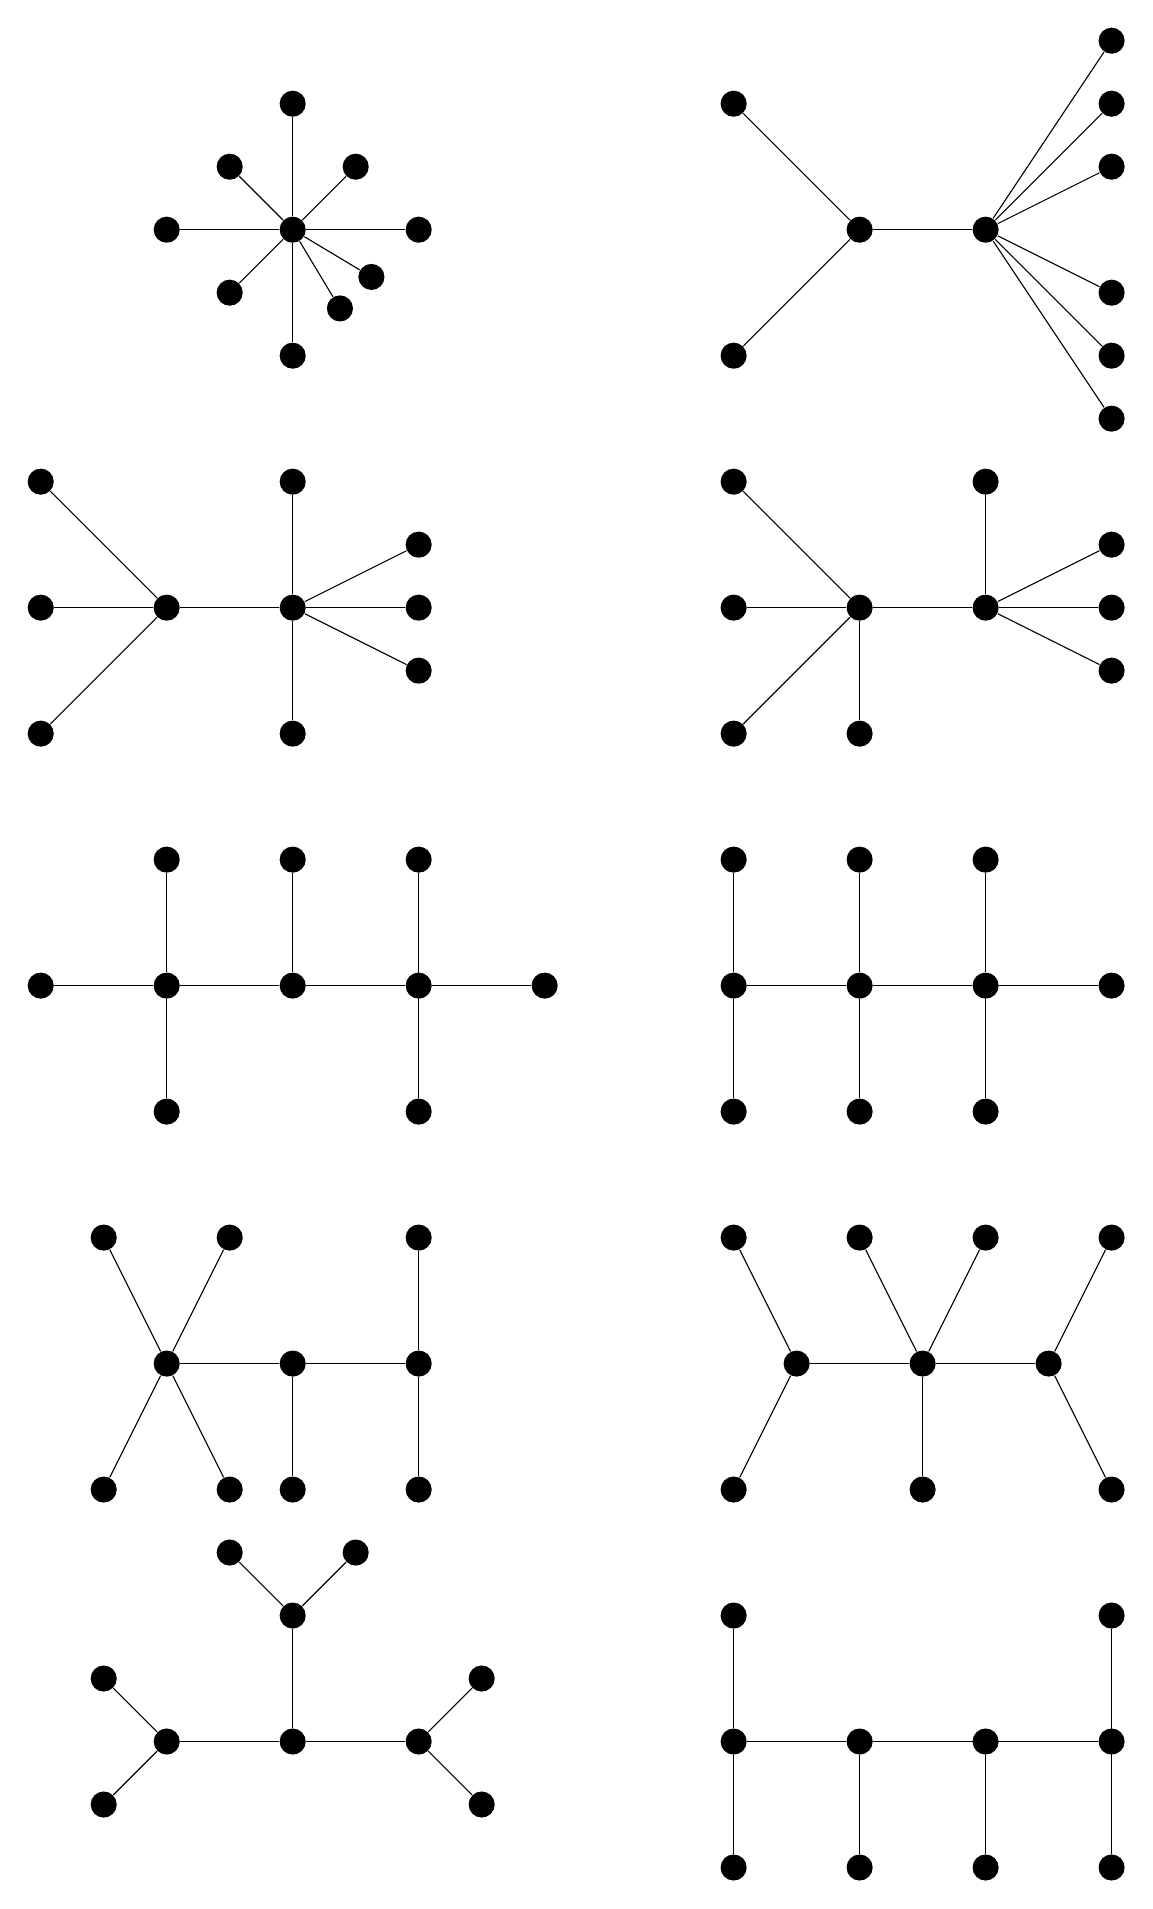
\begin{tikzpicture}[scale = .8]
\node[fill, circle] (A) at (0,0) {}; 
\node[fill, circle] (B) at (2,0) {}; 
\node[fill, circle] (C) at (1,1) {}; 
\node[fill, circle] (D) at (0,2) {}; 
\node[fill, circle] (E) at (-1,1) {}; 
\node[fill, circle] (F) at (-2,0) {}; 
\node[fill, circle] (G) at (-1,-1) {}; 
\node[fill, circle] (H) at (0,-2) {}; 
\node[fill, circle] (I) at (.75,-1.25) {}; 
\node[fill, circle] (J) at (1.25,-.75) {}; 
\draw[-] (A) -- (B);
\draw[-] (A) -- (C);
\draw[-] (A) -- (D);
\draw[-] (A) -- (E);
\draw[-] (A) -- (F);
\draw[-] (A) -- (G);
\draw[-] (A) -- (H);
\draw[-] (A) -- (I);
\draw[-] (A) -- (J);


\begin{scope}[shift={(11,0)}]
\node[fill, circle] (A) at (0,0) {}; 
\node[fill, circle] (B) at (2,3) {}; 
\node[fill, circle] (C) at (2,2) {}; 
\node[fill, circle] (D) at (2,1) {}; 
\node[fill, circle] (E) at (2,-1) {}; 
\node[fill, circle] (F) at (2,-2) {}; 
\node[fill, circle] (G) at (2,-3) {}; 
\node[fill, circle] (H) at (-2,0) {}; 
\node[fill, circle] (I) at (-4,-2) {}; 
\node[fill, circle] (J) at (-4,2) {}; 
\draw[-] (A) -- (B);
\draw[-] (A) -- (C);
\draw[-] (A) -- (D);
\draw[-] (A) -- (E);
\draw[-] (A) -- (F);
\draw[-] (A) -- (G);
\draw[-] (A) -- (H);
\draw[-] (H) -- (I);
\draw[-] (H) -- (J);
\end{scope}
\begin{scope}[shift={(0,-6)}]
\node[fill, circle] (A) at (0,0) {}; 
\node[fill, circle] (B) at (0,2) {}; 
\node[fill, circle] (C) at (2,1) {}; 
\node[fill, circle] (D) at (2,0) {}; 
\node[fill, circle] (E) at (2,-1) {}; 
\node[fill, circle] (F) at (0,-2) {}; 
\node[fill, circle] (G) at (-4,0) {}; 
\node[fill, circle] (H) at (-2,0) {}; 
\node[fill, circle] (I) at (-4,-2) {}; 
\node[fill, circle] (J) at (-4,2) {}; 
\draw[-] (A) -- (B);
\draw[-] (A) -- (C);
\draw[-] (A) -- (D);
\draw[-] (A) -- (E);
\draw[-] (A) -- (F);
\draw[-] (H) -- (G);
\draw[-] (A) -- (H);
\draw[-] (H) -- (I);
\draw[-] (H) -- (J);
\end{scope}
\begin{scope}[shift={(11,-6)}]
\node[fill, circle] (A) at (0,0) {}; 
\node[fill, circle] (B) at (0,2) {}; 
\node[fill, circle] (C) at (2,1) {}; 
\node[fill, circle] (D) at (2,0) {}; 
\node[fill, circle] (E) at (2,-1) {}; 
\node[fill, circle] (F) at (-2,-2) {}; 
\node[fill, circle] (G) at (-4,0) {}; 
\node[fill, circle] (H) at (-2,0) {}; 
\node[fill, circle] (I) at (-4,-2) {}; 
\node[fill, circle] (J) at (-4,2) {}; 
\draw[-] (A) -- (B);
\draw[-] (A) -- (C);
\draw[-] (A) -- (D);
\draw[-] (A) -- (E);
\draw[-] (H) -- (F);
\draw[-] (H) -- (G);
\draw[-] (A) -- (H);
\draw[-] (H) -- (I);
\draw[-] (H) -- (J);
\end{scope}
\begin{scope}[shift={(0,-12)}]
\node[fill, circle] (A) at (0,0) {}; 
\node[fill, circle] (B) at (2,0) {}; 
\node[fill, circle] (C) at (4,0) {}; 
\node[fill, circle] (D) at (-2,0) {}; 
\node[fill, circle] (E) at (-4,0) {}; 
\node[fill, circle] (F) at (-2,-2) {}; 
\node[fill, circle] (G) at (-2,2) {}; 
\node[fill, circle] (H) at (2,2) {}; 
\node[fill, circle] (I) at (2,-2) {}; 
\node[fill, circle] (J) at (0,2) {}; 
\draw[-] (A) -- (B);
\draw[-] (B) -- (C);
\draw[-] (A) -- (D);
\draw[-] (D) -- (E);
\draw[-] (D) -- (F);
\draw[-] (D) -- (G);
\draw[-] (A) -- (J);
\draw[-] (H) -- (I);
\end{scope}
\begin{scope}[shift={(9,-12)}]
\node[fill, circle] (A) at (0,0) {}; 
\node[fill, circle] (B) at (0,2) {}; 
\node[fill, circle] (C) at (0,-2) {}; 
\node[fill, circle] (D) at (-2,0) {}; 
\node[fill, circle] (E) at (-2,-2) {}; 
\node[fill, circle] (F) at (-2,2) {}; 
\node[fill, circle] (G) at (2,0) {}; 
\node[fill, circle] (H) at (2,2) {}; 
\node[fill, circle] (I) at (2,-2) {}; 
\node[fill, circle] (J) at (4,0) {}; 
\draw[-] (A) -- (B);
\draw[-] (A) -- (C);
\draw[-] (A) -- (D);
\draw[-] (D) -- (E);
\draw[-] (D) -- (F);
\draw[-] (A) -- (G);
\draw[-] (G) -- (H);
\draw[-] (G) -- (I);
\draw[-] (G) -- (J);
\end{scope}
\begin{scope}[shift={(0,-18)}]
\node[fill, circle] (A) at (0,0) {}; 
\node[fill, circle] (B) at (2,0) {}; 
\node[fill, circle] (C) at (-2,0) {}; 
\node[fill, circle] (D) at (-1,2) {}; 
\node[fill, circle] (E) at (-1,-2) {}; 
\node[fill, circle] (F) at (-3,2) {}; 
\node[fill, circle] (G) at (-3,-2) {}; 
\node[fill, circle] (H) at (0,-2) {}; 
\node[fill, circle] (I) at (2,-2) {}; 
\node[fill, circle] (J) at (2,2) {}; 
\draw[-] (A) -- (B);
\draw[-] (A) -- (C);
\draw[-] (A) -- (H);
\draw[-] (C) -- (E);
\draw[-] (C) -- (F);
\draw[-] (C) -- (D);
\draw[-] (C) -- (G);
\draw[-] (B) -- (I);
\draw[-] (B) -- (J);
\end{scope}
 \begin{scope}[shift={(10,-18)}]
\node[fill, circle] (A) at (3,2) {}; 
\node[fill, circle] (B) at (1,2) {}; 
\node[fill, circle] (C) at (-3,2) {}; 
\node[fill, circle] (D) at (-1,2) {}; 
\node[fill, circle] (E) at (-2,0) {}; 
\node[fill, circle] (F) at (0,0) {}; 
\node[fill, circle] (G) at (2,0) {}; 
\node[fill, circle] (H) at (3,-2) {}; 
\node[fill, circle] (I) at (0,-2) {}; 
\node[fill, circle] (J) at (-3,-2) {}; 
\draw[-] (A) -- (G);
\draw[-] (B) -- (F);
\draw[-] (C) -- (E);
\draw[-] (D) -- (F);
\draw[-] (E) -- (F);
\draw[-] (F) -- (G);
\draw[-] (H) -- (G);
\draw[-] (F) -- (I);
\draw[-] (E) -- (J);
\end{scope}
 \begin{scope}[shift={(0,-24)}]
\node[fill, circle] (A) at (0,0) {}; 
\node[fill, circle] (B) at (0,2) {}; 
\node[fill, circle] (C) at (-1,3) {}; 
\node[fill, circle] (D) at (1,3) {}; 
\node[fill, circle] (E) at (-2,0) {}; 
\node[fill, circle] (F) at (-3,1) {}; 
\node[fill, circle] (G) at (-3,-1) {}; 
\node[fill, circle] (H) at (2,0) {}; 
\node[fill, circle] (I) at (3,1) {}; 
\node[fill, circle] (J) at (3,-1) {}; 
\draw[-] (A) -- (B);
\draw[-] (B) -- (C);
\draw[-] (B) -- (D);
\draw[-] (A) -- (E);
\draw[-] (E) -- (F);
\draw[-] (E) -- (G);
\draw[-] (A) -- (H);
\draw[-] (H) -- (I);
\draw[-] (H) -- (J);
\end{scope}
 \begin{scope}[shift={(10,-24)}]
\node[fill, circle] (A) at (-3,2) {}; 
\node[fill, circle] (B) at (-3,0) {}; 
\node[fill, circle] (C) at (-3,-2) {}; 
\node[fill, circle] (D) at (-1,0) {}; 
\node[fill, circle] (E) at (-1,-2) {}; 
\node[fill, circle] (F) at (1,0) {}; 
\node[fill, circle] (G) at (1,-2) {}; 
\node[fill, circle] (H) at (3,2) {}; 
\node[fill, circle] (I) at (3,0) {}; 
\node[fill, circle] (J) at (3,-2) {}; 
\draw[-] (A) -- (B);
\draw[-] (B) -- (C);
\draw[-] (B) -- (D);
\draw[-] (D) -- (E);
\draw[-] (D) -- (F);
\draw[-] (F) -- (G);
\draw[-] (D) -- (I);
\draw[-] (H) -- (I);
\draw[-] (H) -- (J);
\end{scope}
\end{tikzpicture}
\end{document}